\section{Auswahl der Technologie und Erstellung des Substrat-Files}
Bevor wir in ADS die Leitungen simulieren können, muss das Substrat-File definiert werden.
Hier lassen sich die Dicke der Kupferleitung sowie die des Dielektrikums FR4 wählen.
\begin{itemize}
    \item FR4: 1~mm
    \item Kupfer: 35\,\textmu m
\end{itemize}
\begin{figure}[H]
    \centering
    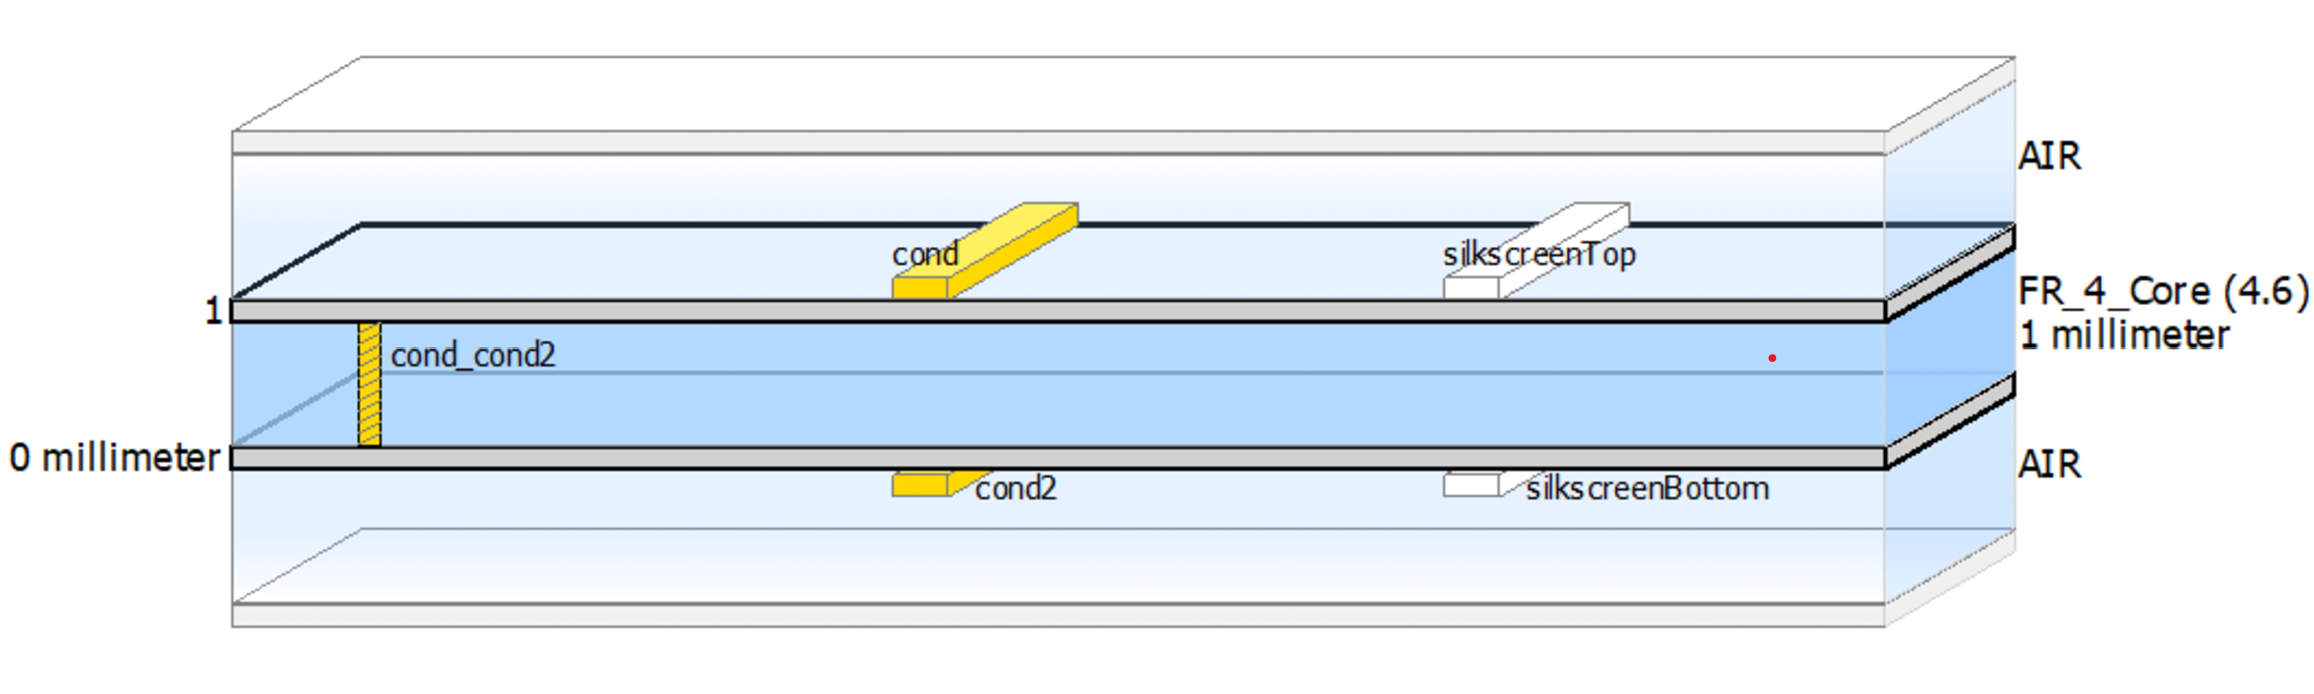
\includegraphics[width=0.9\textwidth]{Pictures/substratFile.png}
    \caption{Substratfile}
\end{figure}

\section{Leitungsdimensionierung}
\subsection{\texorpdfstring{Berechnung der Leitungsbreite ($Z_0 = 50~\Omega$)}{Berechnung der Leitungsbreite (Z0 = 50 Ohm)}}
Nun wird die Leitungsbreite einer Microstrip-Leitung mit der Wellenimpedanz $Z_0 = 50~\Omega$ berechnet.
Dazu werden die Formeln verwendet, die uns auf der Website von Microwaves101, Kapitel Microstrip, zur
Verfügung gestellt werden. Durch eine grobe Abschätzung der Leitungsbreite sieht man, dass folgende Beziehung gilt: \\
\[
\frac{w}{h} \geq 1
\]
$w$ ist hier die Leitungsbreite und $h$ die Höhe des Dielektrikums. In unserem Fall ist $h = 1$~mm und $w$ wird variiert. Die 
effektive Permittivität wird mit folgender Formel berechnet:
\begin{equation}
\varepsilon_e = \frac{\varepsilon_r + 1}{2} + \frac{\varepsilon_r - 1}{2} \left( 1 + 12 \frac{h}{w} \right)^{-\frac{1}{2}}
\end{equation}
$\varepsilon_e$ wird in die Formel zur Leitungsimpedanz eingesetzt. Dabei wird $w$
variiert, bis die Wellenimpedanz $Z_0 = 50~\Omega$ erreicht wird.

Die Formel zur Leitungsimpedanz $Z_0$ lautet:
\begin{equation}
Z_0 = \frac{120 \pi}{\sqrt{\varepsilon_{\text{eff}}} \left( \frac{w}{h} + 1.393 + \frac{2}{3} \ln\left( \frac{w}{h} + 1.444 \right) \right)} \quad \text{(Ohm)}
\end{equation}
Die Berechnung der Leitungsbreite wird hierbei numerisch durchgeführt, da eine analytische Berechnung zu
    
    \begin{table}[H]
        \centering
        \begin{tabular}{|l|l|}
            \hline
            \textbf{Leitungsbreite $w$ (mm)} & \textbf{Wellenimpedanz $Z_0$ ($\Omega$)} \\
            \hline
            1.7 & 52.749 \\
            1.8 & 51.027 \\
            1.9 & 49.419 \\
            2.0 & 47.915 \\
           
            \hline
        \end{tabular}
        \caption{Berechnete Wellenimpedanz für verschiedene Leitungsbreiten}
    \end{table}
    Anhand der berechneten Werte liegt die Leitungsbreite mit $w = 1{,}8~\mathrm{mm}$ am nächsten an der Wellenimpedanz.
    Eine genauere Berechnung ist mit unserem TR nicht möglich. 

       

    \subsection{Verifizierung der berechneten Leitungsbreite}
    Nun wird die Leitungsbreite mithilfe des Controlled Impedance Line Designers simuliert.
    Ziel ist es, $Z_0 = 50~\Omega$ zu erreichen, indem die Leitungsbreite gesweept wird.
    \begin{figure}[H]
        \centering
        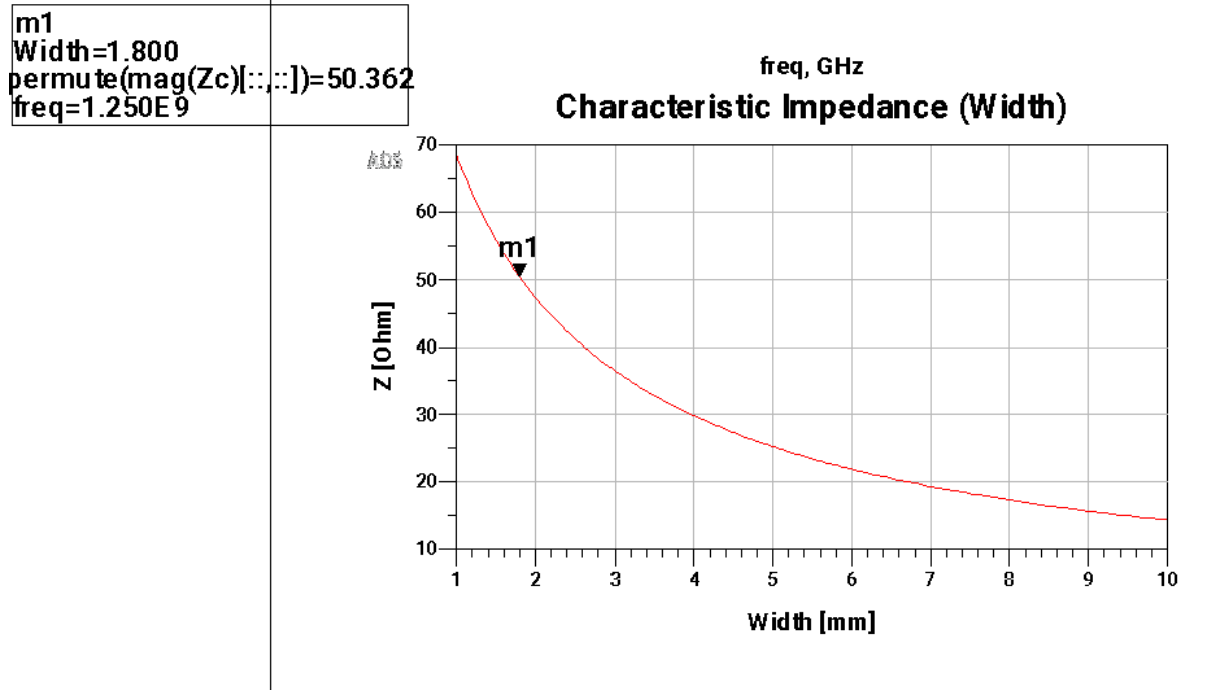
\includegraphics[width=0.8\textwidth]{Pictures/LeitungsbreitenSweep.png}
        \caption{Wellenimpedanz in Abhängigkeit von der Leitungsbreite}
    \end{figure}
    Wie schon numerisch bestimmt, kommen wir mit der Leiterbreite $w=1{,}8~\mathrm{mm}$ der Wellenimpedanz $Z_0 = 50~\Omega$
    am nächsten. Würde man noch genauer sweepen, würde man feststellen, dass die optimale Leiterbreite irgendwo zwischen
    $1{,}8\,\mathrm{mm}$ und $1{,}9\,\mathrm{mm}$ liegt.

\subsection{Charakteristische Länge der Koppelleitungen}
Die Gleichung für die Länge der Leitung wurde schon in Abschnitt~2.2 hergeleitet.
Gegebene Werte:
\begin{align}
    \mu_r &= 1 \\
    c_0 &= 3 \cdot 10^8 \frac{m}{s}
\end{align}

Die Permittivität von Kupfer kann nicht allgemein angegeben werden, sondern muss bestimmt werden. 
Die Permittivität $\epsilon_r = 3{,}42631$ konnte mithilfe des "Controlled Impedance Designers" bestimmt werden. Damit lässt sich die theoretische Leitung berechnen.
\begin{equation}
    L = \frac{c_0}{4 \cdot f_c \cdot \sqrt{\epsilon_r}} = 0{,}03241\,\mathrm{m} = 32{,}41\,\mathrm{mm}
    \label{eq:laenge}
\end{equation}
\clearpage
Mithilfe von ADS wurde die Filtercharakteristik in Abhängigkeit von der Leitungslänge simuliert. Durch das Sweepen der 
Leitungslänge konnten wir folgendes Diagramm erstellen.
\begin{figure}[H]
    \includegraphics[width=0.7\textwidth]{Pictures/SimulationSweepLängeS21.png}
    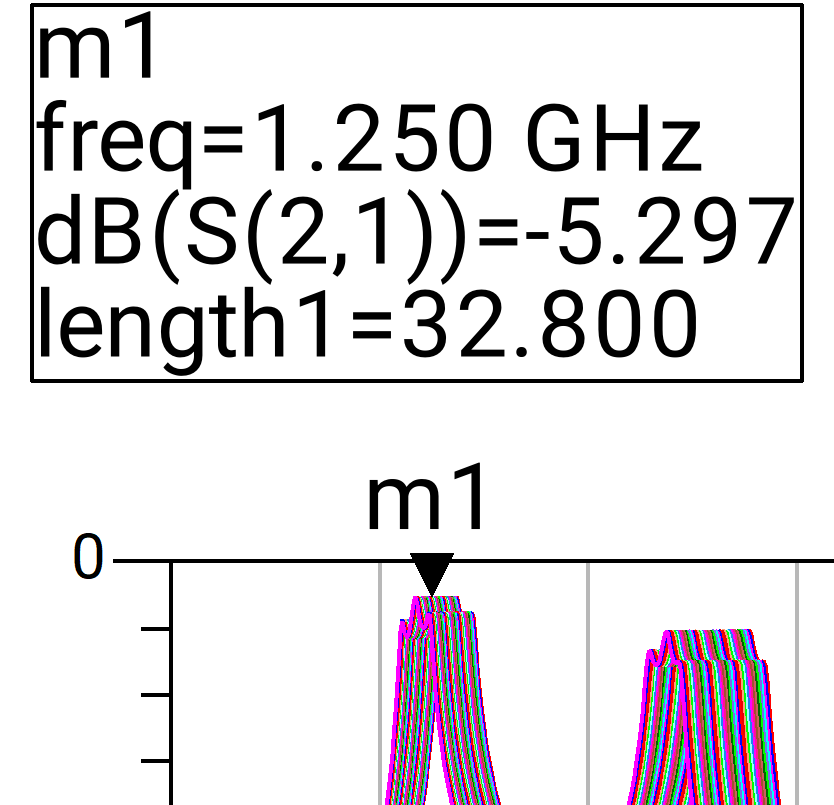
\includegraphics[width=0.3\textwidth]{Pictures/gezoomt.png}
    \centering
    \caption{Leitungslängensweep}
\end{figure}
Schauen wir uns den Filter bei 1,25\,GHz an, sehen wir, dass die beste Filtercharakteristik bei einer
Leitungslänge von etwa $L=32{,}80\,\mathrm{mm}$ liegt.
Das entspricht einer Abweichung von etwa $0{,}4\,\mathrm{mm}$. Dies liegt unter anderem an anderen 
Simulationsmodellen und auch an der Berücksichtigung der vier Bandpassfilter.

\clearpage
\subsection{Simulation im Vergleich zur Praxis}
\begin{figure}[H]
    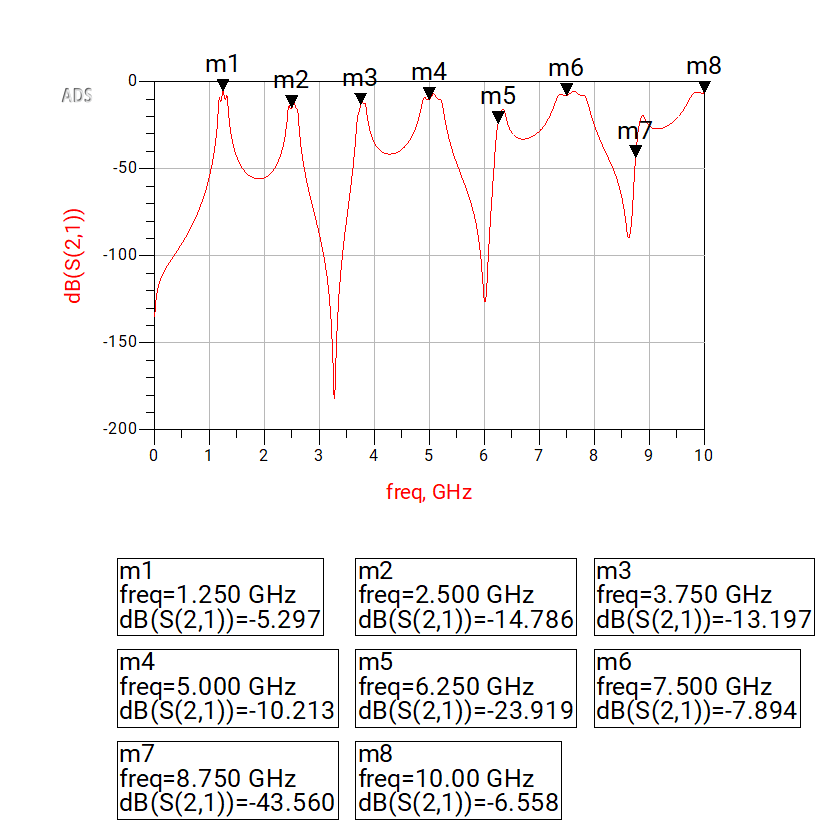
\includegraphics[width=0.7\textwidth]{Pictures/simulationmitmarkern32.8.png}
    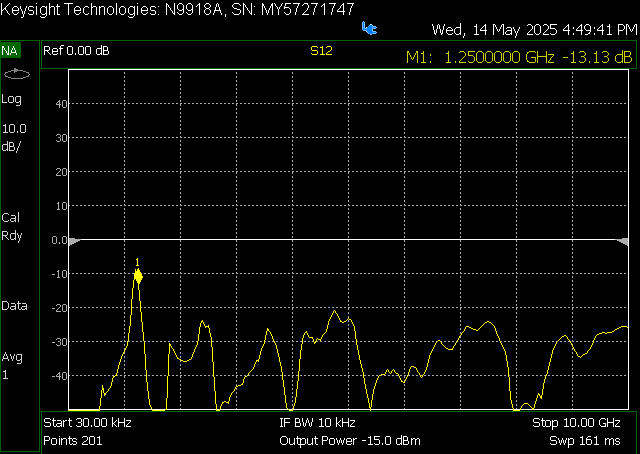
\includegraphics[width=0.7\textwidth]{Pictures/S12neuCooleGrupp.png}
    \centering
    \caption{Filtercharakteristik Praxis vs. Simulation}
\end{figure}
In der Praxis sind, wie in der Theorie, die Peaks, die ein Vielfaches von 1,25\,GHz sind, erkennbar.
Wenn man in der Praxis die 1,25\,GHz genauer anschaut, sieht man, dass der Filter eine Dämpfung von -13,31\,dB
aufweist. In der Theorie jedoch nur -5,23\,dB. Dieser Fehler kommt durch die Dämpfung des Koaxialkabels,
die in der Theorie nicht berücksichtigt wurde.
Nach Versuch 1 ist bekannt, dass die Dämpfung des Koaxialkabels bei 1,25\,GHz etwa -7,13\,dB beträgt.
Wird diese Dämpfung vom theoretischen Wert abgezogen: $D=-5{,}23\,\mathrm{dB}-7{,}13\,\mathrm{dB}=-12{,}36\,\mathrm{dB}$,
kommen wir dem praktischen Wert schon deutlich näher.
     




\section{2.5D EM-Simulation des Coupled-Line-Filters}

Jetzt soll das Coupled-Line-Filter im Schematic aufgebaut werden. 
\subsection{Erstellung und Simulation des Layouts (ohne Knick)}
Dazu wird das Schematic geöffnet und oben im Menü auf "Layout" und dann auf "Generate/Update Layout" geklickt. Dies führt dazu, dass das im Schematic erstellte Schaltbild in das Layout übertragen wird. Es ist festzustellen, dass die Leitungen im Layout tatsächlich erstellt wurden. Dabei ist darauf zu achten, dass die Leitungen korrekt verbunden sind und die Abstände zwischen den Leitungen den Vorgaben entsprechen. Außerdem müssen die Eingangs- und Ausgangsanschlüsse korrekt platziert werden, um eine ordnungsgemäße Simulation der Signalübertragung zu gewährleisten.
Es ergibt sich folgende Ansicht:
\begin{figure}[H]
    \centering
    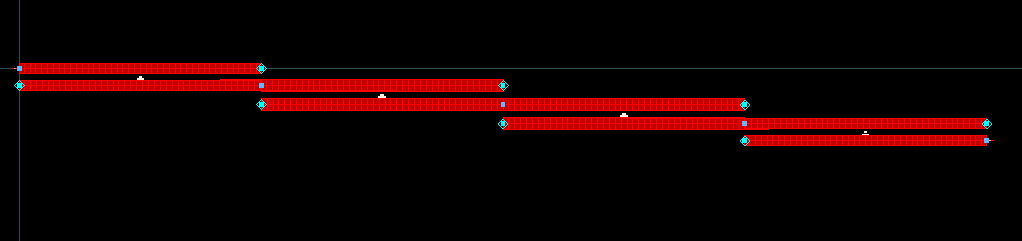
\includegraphics[width=0.8\textwidth]{Pictures/LayoutohneKnick.png}
    \caption{Layout des Coupled-Line-Filters}
\end{figure}

Daraufhin wird die Übertragungsdämpfung des Filters simuliert. Eine elektromagnetische Simulation (EM-Simulation) wird durchgeführt, um die Übertragungsdämpfung des Filters nicht nur eindimensional, sondern auch im 2,5-dimensionalen Raum zu betrachten. 
Dies bedeutet, dass die Simulation in einem physikalischen System geometrisch in 2D beschrieben wird, jedoch dabei elektromagnetische Effekte der dritten Dimension berücksichtigt werden. 
Dies ist in einer Schaltung, die auf Mikrowellen basiert, von großer Bedeutung, da die Signale in der Regel auf Frequenzen im Gigahertz-Bereich arbeiten und die elektromagnetischen Effekte in diesem Bereich signifikant sind. 
Die EM-Simulation ermöglicht es, die Übertragungsdämpfung des Filters unter Berücksichtigung dieser Effekte zu analysieren und zu optimieren.
Nach einer erfolgreichen EM-Simulation entsteht das folgende Dämpfungsdiagramm:
\begin{figure}[H]
    \centering
    \includegraphics[width=0.8\textwidth]{Pictures/EMSimulationohneKnick.png}
    \caption{EM-Simulation des Coupled-Line-Filters}
\end{figure}

Man erkennt deutlich anhand des Diagramms für die S-Parameter S12 bzw. S21, dass die Dämpfung im Bereich von 1,25\,GHz bei gemittelt ca. -11\,dB liegt und die Vielfachen dieser Frequenz auch nicht erheblich gedämpft werden. Dies bestätigt somit das \textbf{Bandpassverhalten} des Filters.
\subsection{Anpassung mit Knick im Layout}
Im Folgenden wird das Layout des Coupled-Line-Filters angepasst, um den Platzbedarf zu verringern. Dazu wird ein Knick in die Microstrip-Leitungen eingefügt.
\subsubsection{Berechnung der Länge des Knicks}
Um den Platzbedarf des Bandpassfilters zu verringern, wird dieser geknickt konstruiert. Dabei sind jedoch einige Aspekte zu beachten:
\begin{itemize}
    \item Die Microstrip-Leitungen müssen als Vielfaches der Wellenlänge ausgelegt werden.
    \item Der Knick bzw. die Ecke kann parasitäre Effekte hervorrufen.
\end{itemize}
Um diese Effekte zu minimieren, kann beispielsweise die Knickkante abgerundet oder die Geometrie der Ecke angepasst werden.

\subsubsection{Anpassung des Schematic und Re-Simulation}
    Das Schematic wird an die neuen Anforderungen mit dem Knick angepasst, damit man die Größe des Filters optimieren kann. Es ergibt sich folgender Aufbau des Schematic:
    \begin{figure}[H]
        \centering
        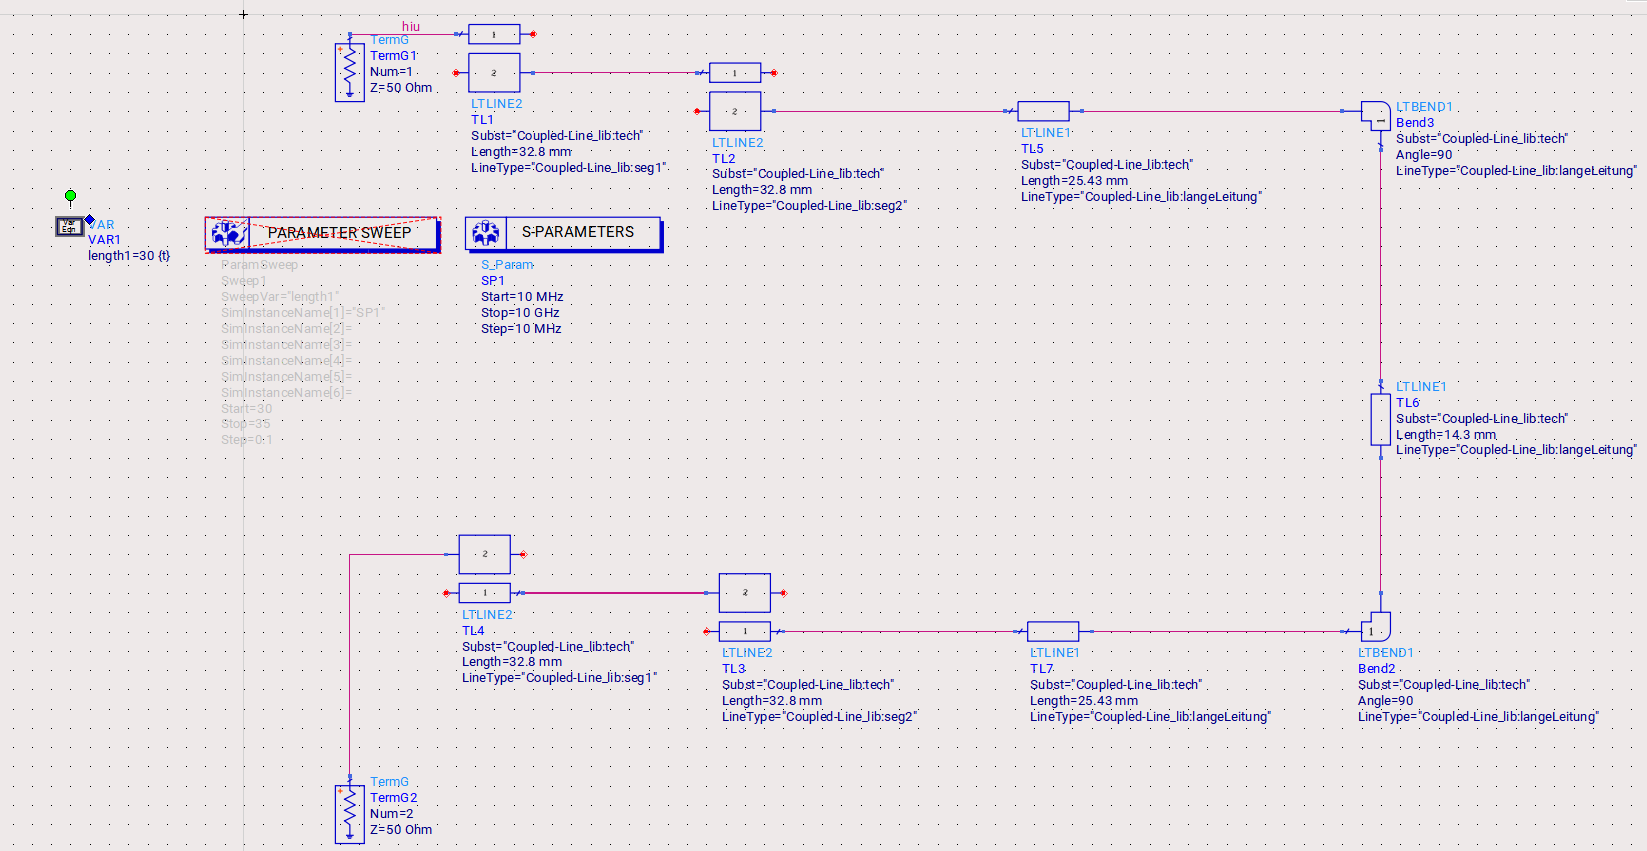
\includegraphics[width=0.8\textwidth]{Pictures/SchematicMitKnick.png}
        \caption{Schematic des Coupled-Line-Filters mit Knick}
    \end{figure}
    Nach dem erneuten Update des Layouts ergibt sich das der echten Schaltung entsprechende Layout:
    \begin{figure}[H]
        \centering
        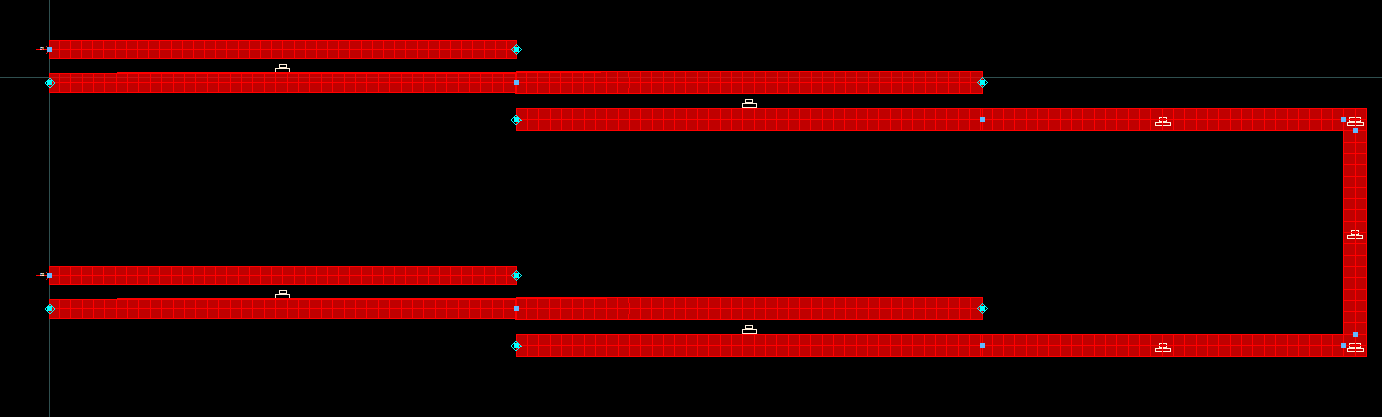
\includegraphics[width=0.8\textwidth]{Pictures/LayoutmitKnick.png}
        \caption{Layout des Coupled-Line-Filters mit Knick}
    \end{figure}
    Daraufhin ergibt sich nach der EM-Simulation des Layouts mit dem Knick folgendes Dämpfungsdiagramm:
    \begin{figure}[H]
        \centering
        \includegraphics[width=0.45\textwidth]{Pictures/EMSimulationohneKnick.png}
        \includegraphics[width=0.45\textwidth]{Pictures/EMSimulationmitKnick.png}
        \caption{EM-Simulation des Coupled-Line-Filters mit Knick (links ohne Knick, rechts mit Knick)}
    \end{figure}

    Jetzt ist zu erkennen, dass die Dämpfung exakt bei 1,25\,GHz und bei den Vielfachen der Basisfrequenz von 1,25\,GHz eine schwächere Dämpfung vorliegt. Dementsprechend wurde die Funktionalität des Bandpassfilters nicht durch den Knick beeinträchtigt.


\subsection{Vergleich der 2.5D EM-Simulation mit der 1D-Simulation}
Man erkennt bei der 1D-Simulation eine viel glattere Dämpfungskurve. Dies liegt daran, dass die 1D-Simulation nur die Übertragungsdämpfung in einer Dimension betrachtet, während die 2.5D EM-Simulation auch die Effekte der dritten Dimension berücksichtigt.
Die 1D-Simulation ist daher weniger realistisch, da sie die komplexen Wechselwirkungen zwischen den Leitungen und den elektromagnetischen Feldern in der dritten Dimension nicht berücksichtigt.
Auch liegt bei der 1D-Simulation der Peak bei der Frequenz von 1,25\,GHz, während bei der 2.5D EM-Simulation der Peak leicht verschoben ist. Dies liegt daran, dass die 2.5D EM-Simulation die realen physikalischen Eigenschaften des Filters besser berücksichtigt und somit eine genauere Darstellung der Übertragungsdämpfung ermöglicht.

Zusammenfassend lässt sich sagen, dass die 1D-Simulation weniger genau ist und in einigen Fällen zu ungenauen Ergebnissen führen kann, insbesondere bei höheren Frequenzen, bei denen die Effekte der dritten Dimension signifikant sind.

\subsection{Auswirkungen auf die S-Parameter}
Wir sehen, dass das S12-Diagramm vom Filter ohne Knick deutlich glatter verläuft als das Diagramm mit Knick.
Das S11-Diagramm mit Knick zeigt eine stärkere Rückreflexion, was auf eine schlechtere Anpassung des Filters
hindeutet.
Begründet ist dies durch den Knick: Dieser erzeugt eine geometrische Diskontinuität, welche parasitäre Kapazitäten und Induktivitäten hervorrufen kann.
Diese verstärken besonders die Signalreflexion.